% !TeX root = thesis.tex
\begin{figure}[ht]
	\begin{subfigure}{.45\textwidth}
		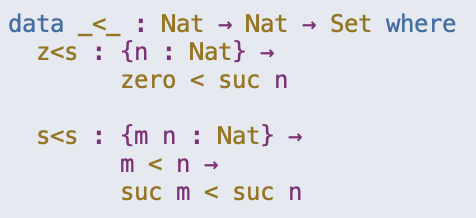
\includegraphics[scale=0.75,valign=t]{imgs/naturals-ordering.png}%
		\caption{Inductive Type Definition}
	\end{subfigure}
	\begin{subfigure}{.45\textwidth}
		\begin{mathpar}
			\Infer{\ZLessThanS}{
				\Gamma \vdash n : Nat
			}{
				\Gamma \vdash z{<}s : zero < suc~ n
			}\\
			\Infer{\SLessThanS}{
				\Gamma \vdash  m : Nat \\ \Gamma \vdash n : Nat \\ \Gamma \vdash p :  m < n
			}{
				\Gamma \vdash s{<}s~p : suc~m < suc~n
			}
		\end{mathpar}
		\caption{Introduction Rules}
	\end{subfigure}
	\caption{Ordering of natural numbers}
	\label{fig:naturals-ordering}
\end{figure}